\section{Planification du projet}
\label{sec:orga}

	Les différents délivrables du projet 4INFO imposent une gestion de projet suivant un modèle de cycle en V. Cependant, nous sommes libres d'adapter nos propres méthodes de développement 

	Ici, nous avons de nombreuses fonctionnalités que nous allons être amenées à réaliser. Il est donc nécessaire de penser à une bonne méthode de gestion lors du développement. Cela nous permettra de gérer au mieux le temps qui nous est imparti en prenant en compte les ressources que nous avons à disposition notamment humaines. D'un côté il est nécessaire d'évaluer l'importance de chaque fonctionnalité, définie bien précisément. De l'autre, la partie la plus complexe, il nous faut estimer la durée pour réaliser chaque tâche.

	En respectant un modèle de cycle en V, nous nous retrouverions donc à développer la plateforme, puis à effectuer différentes séries de tests avant de la délivrer. Le problème de cette méthode est que nous allons devoir faire une sélection de fonctionnalités à développer, s'y tenir,,et un livrable ne sera fournit qu'à la fin. Entre autre, nous ne pourrons pas avoir un retour sur l'application que lorsque le développement sera fini. Il sera impossible d'inférer sur les fonctionnalités puisqu'il n'y aura aucun retour durant le temps de développement. Tout le projet étant étudié, spécifié et conçu en un seul temps, on ne peut pas appliquer ce système pour chaque tâche (on aurait une redondance).

	Cependant, on ne peut pas planifier le développement de l'application en se basant sur les méthodes agiles, tout simplement car il nous est demandé de déterminer les fonctionnalités que nous réaliserons durant la phase de développement et de se tenir à celles-ci. Nous ne nous retrouverons pas à ajouter ou retirer en cours de développement des fonctionnalités ; une gestion agile n'est pas nécessaire. De plus, d'après le retour de Yoann Royer, les proccess agiles sont trop coûteux dans des équipes de moins de huit collaborateurs.

	Pour le processus de développement, on va donc, dans ce rapport, définir une liste non exhaustive de tâches globales (on ne détaille pas encore toutes les sous-tâches de développement qu'une tâche implique, et les tests sont inclus dans le temps de la tâche), et en les ordonnant de manière à obtenir une plateforme qui contiendra au fur et à mesure de plus en plus de fonctionnalités en partant des plus importantes; on arrive au schéma de planification trouvable ci-dessous. L'idée est d'ordonnancer celles-ci suivant l'importance de chaque fonctionnalité, et de pouvoir fournir à plusieurs reprises des versions de la plateforme contenant une nouvelle fonctionnalité 100\% fonctionnelle et complète.

	La première fonctionnalité développée sera la recherche de documents. C'est la fonctionnalité la plus importante, parce que si l'utilisateur doit chercher lui même des documents, l'accès à ceux-ci sera encore plus compliqué qu'actuellement. Le développement sera découpé suivant les options de recherche que l'on souhaite rendre disponible à l'utilisateur; on va donc développer et tester au fur et à mesure des recherches plus complexes en rajoutant des filtres. Cette partie nécessite bien évidemment la mise en place au préalable de la base de données qui sera requêtée. Une version, contenant en plus un très simple visualisation d'une page, sera fournie après le développement de cette fonctionnalité.

	La seconde fonctionnalité va englober toute la consultation des documents. Cette consultation est la fonctionnalité coeur du site, et on va diviser ce développement en plusieurs parties : la visionneuse de documents, la manipulation d'articles, la recherche dans le document, l'architecture de la page et le parcours dans une revue de presse. La manipulation d'articles est une grosse tâche puisqu'elle comprend la gestion de tags et d'ajout de revues dans une revue de presse ainsi que la proposition d'articles proches et de revues de presse associées. Une nouvelle version de la plateforme sera livrée à la fin du développement de la consultation de documents; puisque les deux plus grosses fonctionnalités, et les plus importantes, auront été développées.

	Enfin la gestion et la consultation des revues de presse ainsi que la gestion d'utilisateur et la création de la page d'accueil seront traitées par la suite ; ce sont des fonctionnalités mineures dont le temps de développement nécessaire est plutôt court, notamment car on pourra se baser sur le développement réalisé précédemment pour avancer plus vite. La version finale de la plateforme sera livrée avec la fin du développement de celles-ci. Chacune de ces fonctionnalités ne justifient pas la livraison d'une nouvelle version de l'application.

	À noter que ce planning n'est qu'une première planification du projet décrivant les tâches générales et leur ordonnancement. Le dossier de planification initiale contiendra le planning précis du projet, avec la répartition des ressources disponibles. La durée des tâches pourra être amenée à changer. L'idée ici est de se donner une idée de l'ordre et de la durée de développement des fonctionnalités.

	\begin{figure}[H]
        \centering
        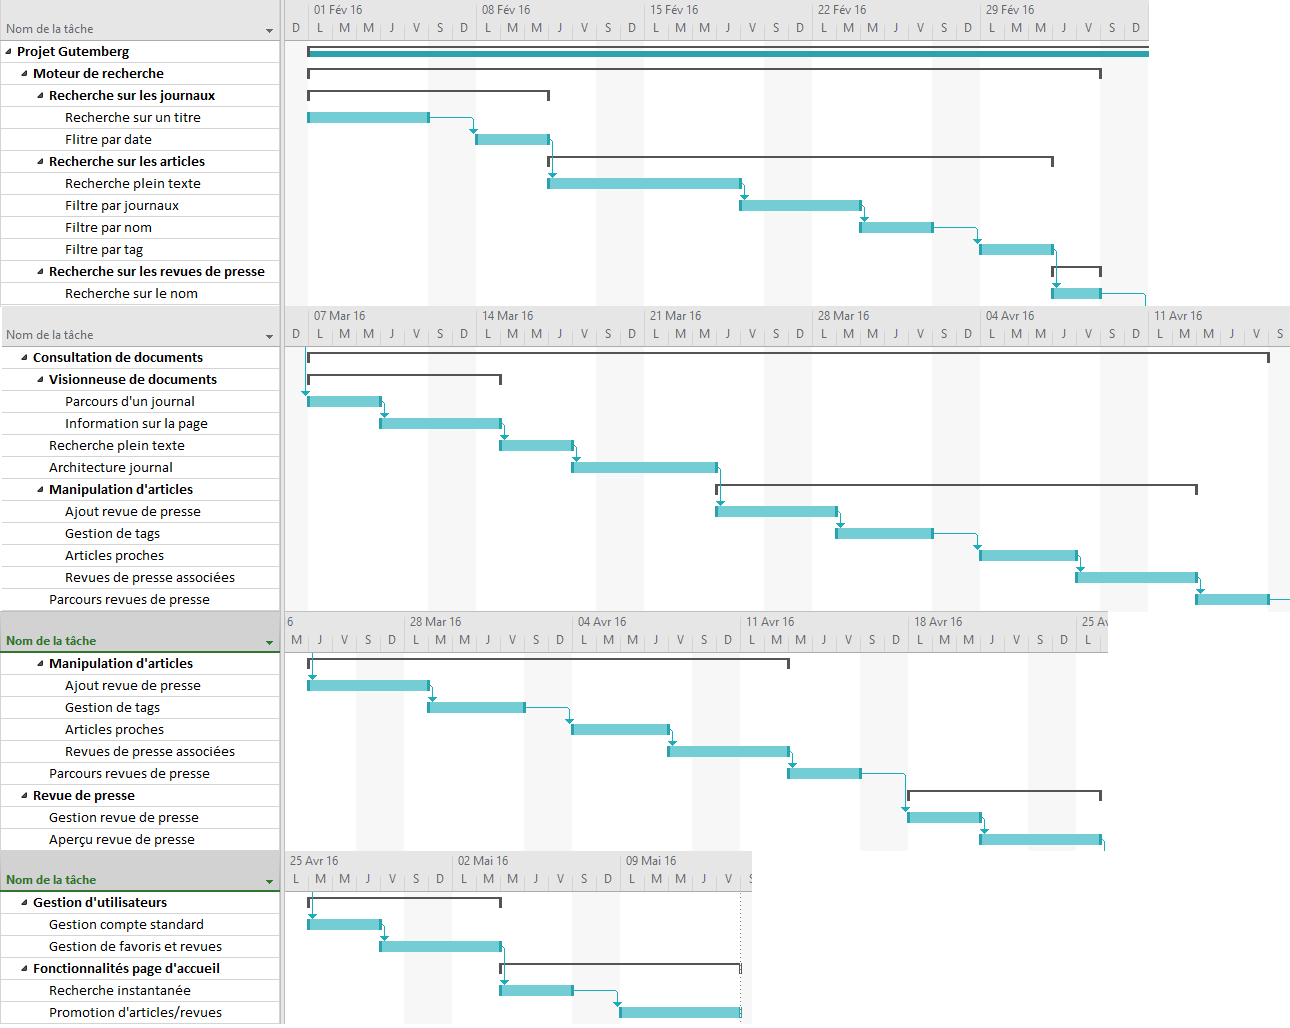
\includegraphics[width=1.3\textwidth, angle=90]{figures/plan.png}
            \caption{Plannification}
            \label{fig:plan_recherche}
    \end{figure}